\section{Experimental and Results}\label{Results}

% \begin{itemize}
%     \item Maxime \ok ? \no ?
%     \item Thierry \ok ? \no ?
%     \item Victor \ok ? \no ?
% \end{itemize}

We have implemented Algorithm \ref{alg:DivideByTheGood} in two different cases and with two different languages : symbolic models and deep learning models using encoded symbolic data. In both settings, we aim to measure the impact of the \tecname. As a consequence the chosen metric will be the efficiency difference with the current treatment of symbolic parameters in batch gradient descent. The public datasets presented in table \ref{tab:datasetChar} will be used for evaluation as well as a private dataset from the supply chain domain.
%% As a consequence we do not compare anything to the state of the art, but we compare established models with their updated version with the \tecname.


\begin{table}[h!] 
  \caption{Datasets characteristics}
  \label{tab:datasetChar}
  \begin{footnotesize}
  \begin{center}
  \begin{tabular}{l|rrrrrrr}
    %%\toprule
    \textbf{Dataset} & Chicago & ACI & compas & DGK  & Forest Cover & KDD99 & UsedCars \\
    \midrule
    instances        & 194m    & 48k & 7.2k   & 72k  & 15k          & 494k  & 38k      \\
    \midrule 
    max cardinality  & 7.9k    & 42  & 341    & 1k & 40             & 66    & 1.1k     \\ 
    \bottomrule		
\end{tabular}
\end{center}
\end{footnotesize}
\end{table}



\subsection{\catmod on public datasets}\label{subsec:public}
\vline


For the \catmod the experiments are run on a supply chain Domain Specific Language: Envision. It is a Python$\cdot$like implementation of SQL narrowed for supply chain problems. A differentiable programming layer on the relational programming language presented in \cite{Peseux2021DifferentiatingRQ} has been added which gives a direct access to the gradients of \catmod. The used programming language is well documented \footnote{\url{https://docs.lokad.com/}} but not open source. %, thus the concerned experiments are not reproducible in the same environment.
For both datasets, we will compare the resulting models resulting from stochastic optimization based on Adam or our algorithm for the determination of the parameters of a linear regression model, slightly modified to take into account symbolical variables. To implement this idea, we worked on two different public datasets : the Chicago taxi ride dataset and the Belarus used car dataset.

The Chicago taxi rides dataset that can be found here \footnote{\url{https://data.cityofchicago.org/Transportation/Taxi-Trips/wrvz-psew}}. 
For each ride, we use the taxi identifier, distance, payment type and the tips amount. We use modified version of linear regression to predict the tip based on the trip distance and the payment type. We used a symbolic version of this model where the slope depends on the taxi and the payment method, the intercept remains shared among all the trips, presented in Equation \ref{eq:otherModel}:
\begin{equation*}\label{eq:otherModel}
    \hat{tips} = (\gamma_{\text{taxi}} \times \mu_{\text{payment}}) \times distance + b 
\end{equation*}
There is one $\gamma$ per taxi and also one $\mu$ per payment method, this is a \catmod. As the intercept is shared among all taxis, the dataset is unsplitable. A model based on Equation \ref{eq:splitable}
\begin{equation}\label{eq:splitable}
\hat{tips} = \gamma_{\text{taxi}}  \times distance + b_{taxi}
\end{equation}
could be split in different dataset (one per taxi) and thus we would be in the classical setting of a linear regression.



We also worked on the Belarus used cars dataset. It is presented presented by \cite{UsedCars} and contains vehicle features. We take into account the car manufacturer, the production year, the origin region of the car to predict the selling price of the car as presented in Equation \ref{eq:otherModelUsedCars}.
\begin{equation*}\label{eq:otherModelUsedCars}
    \hat{price} = (\gamma_{\text{manufacturer}} \times \mu_{\text{region}}) \times year + b 
\end{equation*}

As seen table \ref{tab:envisionResult}, the relational batch performed better with our proposition based on Algorithm \ref{alg:DivideByTheGood} with the following setting: 30 epochs ; optimizer Adam with default setting ; batch size of 1. Experiment was reproduced 20 times. The used metric is the mean square error (MSE).
\begin{table}[h!]% h asks to places the floating element [h]ere.
  \caption{Results with \catmod }
  \label{tab:envisionResult}
  \begin{footnotesize}
  \begin{center}
  \begin{tabular}{l|cc}
    \toprule
    Dataset      & Adam         & Adam \& \tecnameAbrv       \\
    \midrule                                                                                     
    Chicago Ride & 35.58 $\pm$ 1.11 & \bold{9.45 $\pm$ 16.33} \\
    Used Cars & 7.10 $\pm$ 2.45 & \textbf{0.08 $\pm$ 0.01} \\
  \bottomrule
\end{tabular}
\end{center}
\end{footnotesize}
\end{table}


% %%%%%%%%%%%%%%%%%%%%%%%%%%%%%%%%%%%%%%%%%%%%%%%%%%%%%%%%%%%%%%%%
% %%%%%%%%%%%%%%%%%%%%%%%%%%%%%%%%%%%%%%%%%%%%%%%%%%%%%%%%%%%%%%%%
% %%%%%%%%%%%%%%%%%%%%%%%%%%%%%%%%%%%%%%%%%%%%%%%%%%%%%%%%%%%%%%%%

\subsection{\catmod on a real case}
\TODO validate it with Joannes/Victor

We have successfully deployed to production such \catmod at Lokad, a french company specialized in supply chain optimization, in order to weekly forecast sales of a large retail company. The forecast is done at the item level. The dataset contains 3 years of history and concerns more than $13$ millions different items.

The implemented \catmod is similar\footnote{we do not disclose the actual model for confidentiality reasons.} to:

%%\begin{equation*}
\begin{align*}
    \hat{y}(item, week) = \quad &\theta_{store(item)} \times \theta_{color(item)} \times \theta_{size(item)} \times\\
      & \Theta [group(item), WeekNumber(week)]
\end{align*}
%%\end{equation*}

$\Theta [group(item), WeekNumber(week)]$ is a parameter vector that can be seen as a function that aims to capture the annual seasonality for a given group of items:
\begin{equation*}
    \Theta : Groups \times [| 1, 52|] \longrightarrow \mathbb{R}
\end{equation*}

We use Adam as optimizer with its default values with \tecname and a minibatch of $1$ to update the parameters. It outstandingly outperforms the classical gradient estimator on this (very) \catmod. The final loss (decayed RMSE) is an order of magnitude better with \tecname on the testing dataset.


\subsection{Deep Learning}

For the Deep Learning models, we applied our solution on \textbf{PyTorch}. On this framework, it very easy to update every parameter gradient according to Algorithm \ref{alg:DivideByTheGood}. The code is available and \href{https://github.com/ppmdatix/RelationalBatch}{experiments can be found here}\footnote{https://github.com/ppmdatix/RelationalBatch}.  In order to evaluate the impact of our proposal,  we worked on 4 different symbolic datasets :

the Adult Census Income (ACI) dataset presented in \cite{incomeDataset} that aims to predict wealth category of individuals. The Compas dataset contains information on criminal defendant’s likelihood of re-offending.  The Forest Cover dataset presented \cite{ForestCover} contains symbolic characteristics on $30m^2$ forest cells. The objective is to predict the forest cover type. The KDD99 dataset accessible by \cite{KDD99} and aims to predict cyber-attacks. Finally the used Cars datasets from Belarus presented in \ref{subsec:public}.


%%The Don't Get Kicked (DGK) dataset introduced by \cite{DGK}. The objective is to predict if the car purchased at the Auction is a good or a bad buy.



In order to only measure the impact of the \tecname, we \textit{only} use those symbolic variables in our experiments. Those datasets tasks are quiet easy. As a consequence we use a very small network to highlight our approach. Our network is made of 3 dense layers of sizes $[4,8,4]$ with a batch of size $128$. We also perform experiments on a ResNet-like network that give same results. We use the $l_2$ loss. We also used the same ResNet-like network than \cite{RevisitingDeepForTabular}.
We have tested three different optimizer with their default settings: SGD (vanilla), Adagrad and Adam.

Results are reproducible in the repository and are recorded in Tables \ref{tab:resultsMLP32} \ref{tab:resultsRESNET32} \ref{tab:resultsMLP64} \ref{tab:resultsRESNET64} \ref{tab:resultsMLP128}  \ref{tab:resultsRESNET128} \ref{tab:resultsMLP256} \ref{tab:resultsRESNET256} \ref{tab:resultsMLP512} \ref{tab:resultsRESNET512} \ref{tab:resultsMLP1024}      \ref{tab:resultsRESNET1024} in appendices. On the different datasets we have worked on, we always see an improvement of the loss on the testing dataset using the \tecname. A specific focus on the ACI dataset is done in Figure \ref{fig:ACIresults}.
This proves the need to specifically handle stochastic gradient on symbolic data. Results in different settings demonstrate the advantage to use \tecname whatever the optimizer. Among other things, AdaGrad tries to handle gradient on sparse data (which includes one-hot encoded data) but we see a clear improvement on that task.



\begin{figure}[h!]
  \centering
  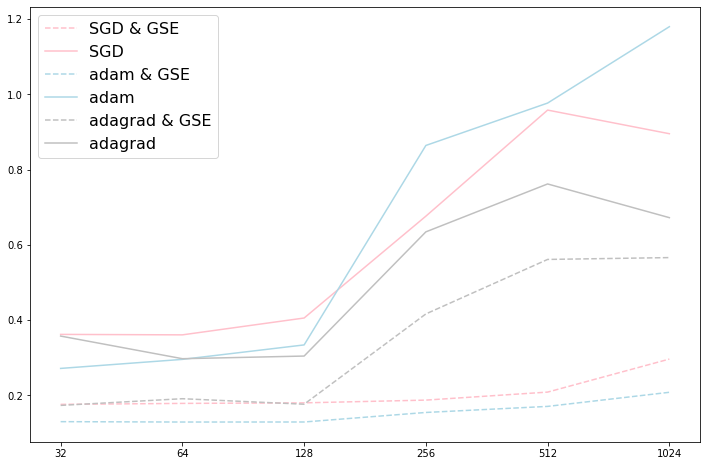
\includegraphics[width=0.7\linewidth]{figures/AdultIncomelossResults.png}
  \caption{Results on the ACI dataset. The dashed curves represents experiments wit \tecnameAbrv  and shows an improvement on the loss for every optimizer used.}
  \label{fig:ACIresults}
\end{figure}


% On top that, we clearly see that \tecname leads to greater variance in our results. Our intuition on it is that we estimate the gradient with less observation as written on line 17 ( $\rhd$ \textcolor{blue}{scaled gradient} ) of Algorithm \ref{alg:DivideByTheGood}.


